%%%%%%%%%%%%%%%%%%%%%%%%%%%%%%%%%%%%%%%%%
% "ModernCV" CV and Cover Letter
% LaTeX Template
% Version 1.3 (29/10/16)
%
% This template has been downloaded from:
% http://www.LaTeXTemplates.com
%
% Original author:
% Xavier Danaux (xdanaux@gmail.com) with modifications by:
% Vel (vel@latextemplates.com)
%
% License:
% CC BY-NC-SA 3.0 (http://creativecommons.org/licenses/by-nc-sa/3.0/)
%
% Important note:
% This template requires the moderncv.cls and .sty files to be in the same 
% directory as this .tex file. These files provide the resume style and themes 
% used for structuring the document.
%
%%%%%%%%%%%%%%%%%%%%%%%%%%%%%%%%%%%%%%%%%

%----------------------------------------------------------------------------------------
%	PACKAGES AND OTHER DOCUMENT CONFIGURATIONS
%----------------------------------------------------------------------------------------

\documentclass[11pt,a4paper,sans]{moderncv} % Font sizes: 10, 11, or 12; paper sizes: a4paper, letterpaper, a5paper, legalpaper, executivepaper or landscape; font families: sans or roman

\newcommand\tab[1][1cm]{\hspace*{#1}}

\moderncvstyle{casual} % CV theme - options include: 'casual' (default), 'classic', 'oldstyle' and 'banking'
\moderncvcolor{blue} % CV color - options include: 'blue' (default), 'orange', 'green', 'red', 'purple', 'grey' and 'black'


\usepackage{booktabs}
\usepackage[scale=0.75]{geometry} % Reduce document margins
\usepackage[final]{pdfpages}

\definecolor{cvcolor}{RGB}{56, 115, 178}


%\setlength{\hintscolumnwidth}{3cm} % Uncomment to change the width of the dates column
%\setlength{\makecvtitlenamewidth}{10cm} % For the 'classic' style, uncomment to adjust the width of the space allocated to your name

%----------------------------------------------------------------------------------------
%	NAME AND CONTACT INFORMATION SECTION
%----------------------------------------------------------------------------------------

\firstname{Dario} % Your first name
\familyname{Gangi} % Your last name

\setlength\tabcolsep{6pt}

% All information in this block is optional, comment out any lines you don't need
\title{Curriculum Vitae}
\address{Piazzale Marconi, 5}{27058 - Voghera (PV) - Italia}
\mobile{(+39) 333 6567094}
%\phone{(000) 111 1112}
%\fax{(000) 111 1113}
\email{dariogangi@hotmail.com}
%\homepage{staff.org.edu/~jsmith}{staff.org.edu/$\sim$jsmith} % The first argument is the url for the clickable link, the second argument is the url displayed in the template - this allows special characters to be displayed such as the tilde in this example
%\extrainfo{additional information}
\photo[70pt][0.4pt]{pictures/foto} % The first bracket is the picture height, the second is the thickness of the frame around the picture (0pt for no frame)
%\quote{"A witty and playful quotation" - John Smith}

%----------------------------------------------------------------------------------------

\begin{document}

%----------------------------------------------------------------------------------------
%	CURRICULUM VITAE
%----------------------------------------------------------------------------------------

\makecvtitle % Print the CV title

\section{INFORMAZIONI PERSONALI}
\textbf{Nome}: \hspace{8mm} Dario Gangi
\\
\textbf{Indirizzo}: \hspace{4mm} Piazzale Marconi, 5 - 27058 Voghera (PV)
\\
\textbf{Cellulare}: \hspace{4.5mm} (+39) 333 65 67 094
\\
\textbf{Email}: \hspace{9mm} dariogangi@hotmail.com
\\
\textbf{Skype}: \hspace{8.5mm} dario.gangi

%----------------------------------------------------------------------------------------
%	WORK EXPERIENCE SECTION
%----------------------------------------------------------------------------------------

\section{ESPERIENZE}

\subsection{Lavorative}

\cventry{11/2008--01/2011}{Programmatore}{Elemental srl}{Viale Ippocrate, 73, 00161 - Roma (Italia)}{}
{
	\textbf{Attivit\`{a} o settore:} Game Development
	\newline{}
	\url{http://www.elementaldesign.it/}
	\newline{}
	\url{http://www.aiv01.it/} 
	\begin{itemize}
		\item Programmazione C\#
		\item Utilizzo delle librerie grafiche XNA
		\begin{itemize}
			\item Gestione 3D delle telecamere (principalmente orbital camera, third person camera)
			\item Implementazione dell'algoritmo Convex Hull per la creazione di mesh fisiche
			\item Gestione della GUI
			\item Implementazione di collisione con un tronco di piramide per il Frustum Culling
			\item Implementazione di A* per l'intelligenza artificiale dei nemici
		\end{itemize}
		\item Programmazione di gameplay del gioco Evil Heroes
		\begin{itemize}
			\item Playlist di video di gameplay:
			\newline{}
			\url{https://www.youtube.com/playlist?list=PL3bhmuxOZlohK9x4cdzjEwoKqdPXbryAy}
			\item Spostamento dei nemici verso il personaggio principale
			\item Implementazione della barra vitale del personaggio principale
		\end{itemize}
	\end{itemize}
}

\cventry{11/2012--04/2013}{Programmatore}{Centro di Ricerca C.A.T.T.I.D. Universit\`{a} degli Studi "La Sapienza"}{Roma}{}
{
	\begin{itemize}
		\item Tirocinio per Corso di Laurea Triennale in Informatica
		\item Sviluppo di un'applicazione per Windows Phone 7
		\item Utilizzo di C\# e Windows Phone SDK 7.1
	\end{itemize}
}


\subsection{Formative}

\cventry{04/2014--06/2014}{Programmatore}{Universit\`{a} degli Studi "La Sapienza"}{Roma}{}
{
	\url{http://www.electricitylab.net/blog/9-news/46-differenziati-un-tuo-gesto-migliorera-il-mondo.html}
	\newline{}
	\url{http://gamificationlab.uniroma1.it/laboratorio/progetto-gamificationlab-2014}
	\begin{itemize}
		\item Sviluppo di un piccolo gioco sulla raccolta differenziata
		\item Utilizzo di C\#, Unity 4, Arduino, Kinect for Windows SDK
		\item Presentazione alla fiera Maker Faire di Roma
		\newline{} \url{http://gamificationlab.uniroma1.it/archivionotizie/il-prototipo-del-gioco-differenziati-selezionato-alla-maker-faire}
	\end{itemize}
}

\cventry{05/2014--09/2014}{Programmatore}{Universit\`{a} degli Studi "La Sapienza"}{Roma}{}
{
	\begin{itemize}
		\item Sviluppo di un'applicazione Android per il Museo di Antropologia "Giuseppe Sergi" di Roma
		\item Utilizzo del motore grafico Unity 4
		\item Implementazione di un'activity per la visualizzazione di modelli 3D di crani esposti al museo
		\item Pubblicazione su Google Play
		\newline{}
		\url{https://play.google.com/store/apps/details?id=sapienza.informatica.man}
	\end{itemize}
}

\cventry{02/2016--10/2016}{Programmatore}{Laboratorio di Visione Artificiale VisionLab (Universit\`{a} degli Studi "La Sapienza")}{Roma}{}
{
	\begin{itemize}
		\item Sviluppo di un sistema di sorveglianza attiva commissionato dal Ministero della Difesa
		\item Utilizzo di OpenCV e linguaggio C++
	\end{itemize}
}

%----------------------------------------------------------------------------------------
%	EDUCATION SECTION
%----------------------------------------------------------------------------------------

\section{ISTRUZIONE}
\cventry{2001--2006}{Diploma di Ragioniere Programmatore}{ITC Paolo Dagomari}{Via di Reggiana, 86, 59100 - Prato (Italia)}{}
{
	%\url{http://www.itesdagomari.it/ }
}


\cventry{2007--2013}{Laurea Triennale in Informatica}{Universit\`{a} degli Studi "La Sapienza"}{Via Salaria, 113, 00198 - Roma (Italia)}
{
	\newline{}
	\textit{\textbf{Votazione conseguita:} 103/110}
}
{
%\url{http://www.studiareinformatica.uniroma1.it}
	\begin{itemize}
		\item Conoscenze matematiche avanzate
		\item Conoscenze di programmazione in C e Java
		\item Conoscenze di linguaggi funzionali
		\item Conoscenze base sull'architettura di rete, modelli ISO-OSI e TCP/IP
		\item Conoscenze a basso livello nei sistemi operativi UNIX
		\item Conoscenze dell'architettura di un elaboratore
		\item Conoscenze riguardo la progettazione e l'analisi di un software
		\item Conoscenze teoriche e pratiche riguardo le basi di dati
		\item Progettazione e analisi di algoritmi
	\end{itemize}
}


\cventry{2007--2008}{Certificato in Videogame Programming}{Accademia Italiana Videogiochi}{Viale Ippocrate, 73, 00161 - Roma (Italia)}{}
{
	%\url{http://www.aiv01.it}
	\begin{itemize}
		\item Programmazione in linguaggi C\textbackslash C++
		\item Programmazione in linguaggio C\# Orientato a Oggetti
		\item Utilizzo di Microsoft Visual Studio 2007/2010
		\item Utilizzo di sistemi di software di controllo versione CVS, SVN e Microsoft Team Foundation Version Control
		\item Programmazione con DirectX 9.0c
		\item Programmazione di pixel shader e vertex shader con linguaggio HLSL
	\end{itemize}
}


\cventry{2013--2016}{Laurea Magistrale in Informatica}{Universit\`{a} degli Studi di Roma "La Sapienza"}{Via Salaria, 113, 00198 - Roma (Italia)}
{
	\newline{}
	\textit{\textbf{Votazione conseguita:} 110 e lode/110}
}
{
	%\url{http://www.studiareinformatica.uniroma1.it}
	\begin{itemize}
		\item Studio e programmazione in ambito della grafica computazionale (algoritmo di ray tracing, pipeline grafica, OpenGL, GLSL)
		\item Elaborazione delle immagini nell'ambito della visione artificiale e dei sistemi biometrici (utilizzo di OpenCV)
		\item Studio nell'ambito dell'Information Retrivial (utilizzo delle Twitter API, tramite Twitter4j)
		\item Studio di Big Data e utilizzo di Hadoop tramite Amazon Web Service
		\item Studio nell'ambito dell'informatica teorica (calcolabilit\`{a}, complessit\`{a}, lambda calcolo)
		\item Studio nell'ambito della gamification e utilizzo del motore graficio Unity
		\item Studio dell'interazione tra uomo e macchina, anche tramite sistemi multimodali
		\item Studio approfondito sulla progettazione, gestione delle reti e cloud computing
		\item Studio teorico e applicazione pratica di varie tecniche di Machine Learning
	\end{itemize}
}

\section{TESI DI LAUREA MAGISTRALE}

\cvitem{Titolo}{\emph{Un Sistema per l'Analisi dei Cambiamenti in Immagini Acquisite da UAV per la Sorveglianza Attiva}}
\cvitem{Relatore}{Professore Luigi Cinque}
\cvitem{Descrizione}{Progettazione e sviluppo di un sistema di sorveglianza attiva che ha l'obiettivo di rilevare dei cambiamenti, in particolare in ambienti outdoor non urbani. Tale sistema dovr\`{a} analizzare le immagini aeree acqusite da un drone UAV che monitora una specifica zona. Il sistema \`{e} stato sviluppato in linguaggio C++ con l'ausilio della libreria OpenCV.}

%----------------------------------------------------------------------------------------
%	COMMUNICATION SKILLS SECTION
%----------------------------------------------------------------------------------------

\section{COMPETENZE COMUNICATIVE}

\cvitem{}{Buone competenze comunicative in team di sviluppo acquisite grazie alle esperienze lavorative.}
\cvitem{}{Buone capacit\`{a} di comunicazione davanti a un pubblico di persone, acquisite durante alcune presentazioni e conferenze in ambito universitario.}


%----------------------------------------------------------------------------------------
%	COMPUTER SKILLS SECTION
%----------------------------------------------------------------------------------------

\section{COMPETENZE PROFESSIONALI}

\cvitem{Completa}{C\textbackslash C++, C\#}
\cvitem{Avanzata}{Java}
\cvitem{Buone\textbackslash Ottime}{Unity 3D, OpenCV, Microsoft .Net, Microsoft Visual Studio, XNA, Windows Phone SDK, NetBeans, Eclipse, \LaTeX}
\cvitem{Sufficiente}{OpenGL, Boost C++, DirectX, HLSL, GLSL, Twitter4j, SQL, Linguaggi funzionali, Programmazione Assembly di architetture MIPS R2000/R3000, Android SDK, Cisco IOS, Amazon Web Services, Hadoop}

\clearpage
%----------------------------------------------------------------------------------------
%	LANGUAGES SECTION
%----------------------------------------------------------------------------------------

\section{CONOSCENZE LINGUISTICHE}

\cvitemwithcomment{Lingua Madre}{Italiano}{}

\cvitemwithcomment{Inglese}
{%
	\centering
	\begin{tabular}{*{5}{c}}
		\toprule
		\multicolumn{2}{c}{\textcolor{cvcolor}{COMPRENSIONE}} & \multicolumn{2}{c}{\textcolor{cvcolor}{PARLATO}}          & \textcolor{cvcolor}{PRODUZIONE SCRITTA} \\ \midrule
		& & \textcolor{cvcolor}{Interazione} & \textcolor{cvcolor}{Produzione} & \\
		\textcolor{cvcolor}{Ascolto}         & \textcolor{cvcolor}{Lettura}        &  \textcolor{cvcolor}{Orale} &  \textcolor{cvcolor}{Orale} & -       \\             B1                & B2              & B1                 & B1                & B2      \\ \bottomrule
	\end{tabular}%
}{}

\cvitemwithcomment{Tedesco}
{%
	\centering
	\begin{tabular}{*{5}{c}}
		\toprule
		\multicolumn{2}{c}{\textcolor{cvcolor}{COMPRENSIONE}} & \multicolumn{2}{c}{\textcolor{cvcolor}{PARLATO}}          & \textcolor{cvcolor}{PRODUZIONE SCRITTA} \\ \midrule
		& & \textcolor{cvcolor}{Interazione} & \textcolor{cvcolor}{Produzione} & \\
		\textcolor{cvcolor}{Ascolto}         & \textcolor{cvcolor}{Lettura}        &  \textcolor{cvcolor}{Orale} &  \textcolor{cvcolor}{Orale} & -       \\             A1                & A1              & A1                 & A1                & A1      \\ \bottomrule
	\end{tabular}%
}{}

%----------------------------------------------------------------------------------------
%	INTERESTS SECTION
%----------------------------------------------------------------------------------------

\section{Interessi}

\renewcommand{\listitemsymbol}{-~} % Changes the symbol used for lists

\cvlistdoubleitem{Retrogaming}{Informatica}
\cvlistdoubleitem{Cinema}{}

%----------------------------------------------------------------------------------------

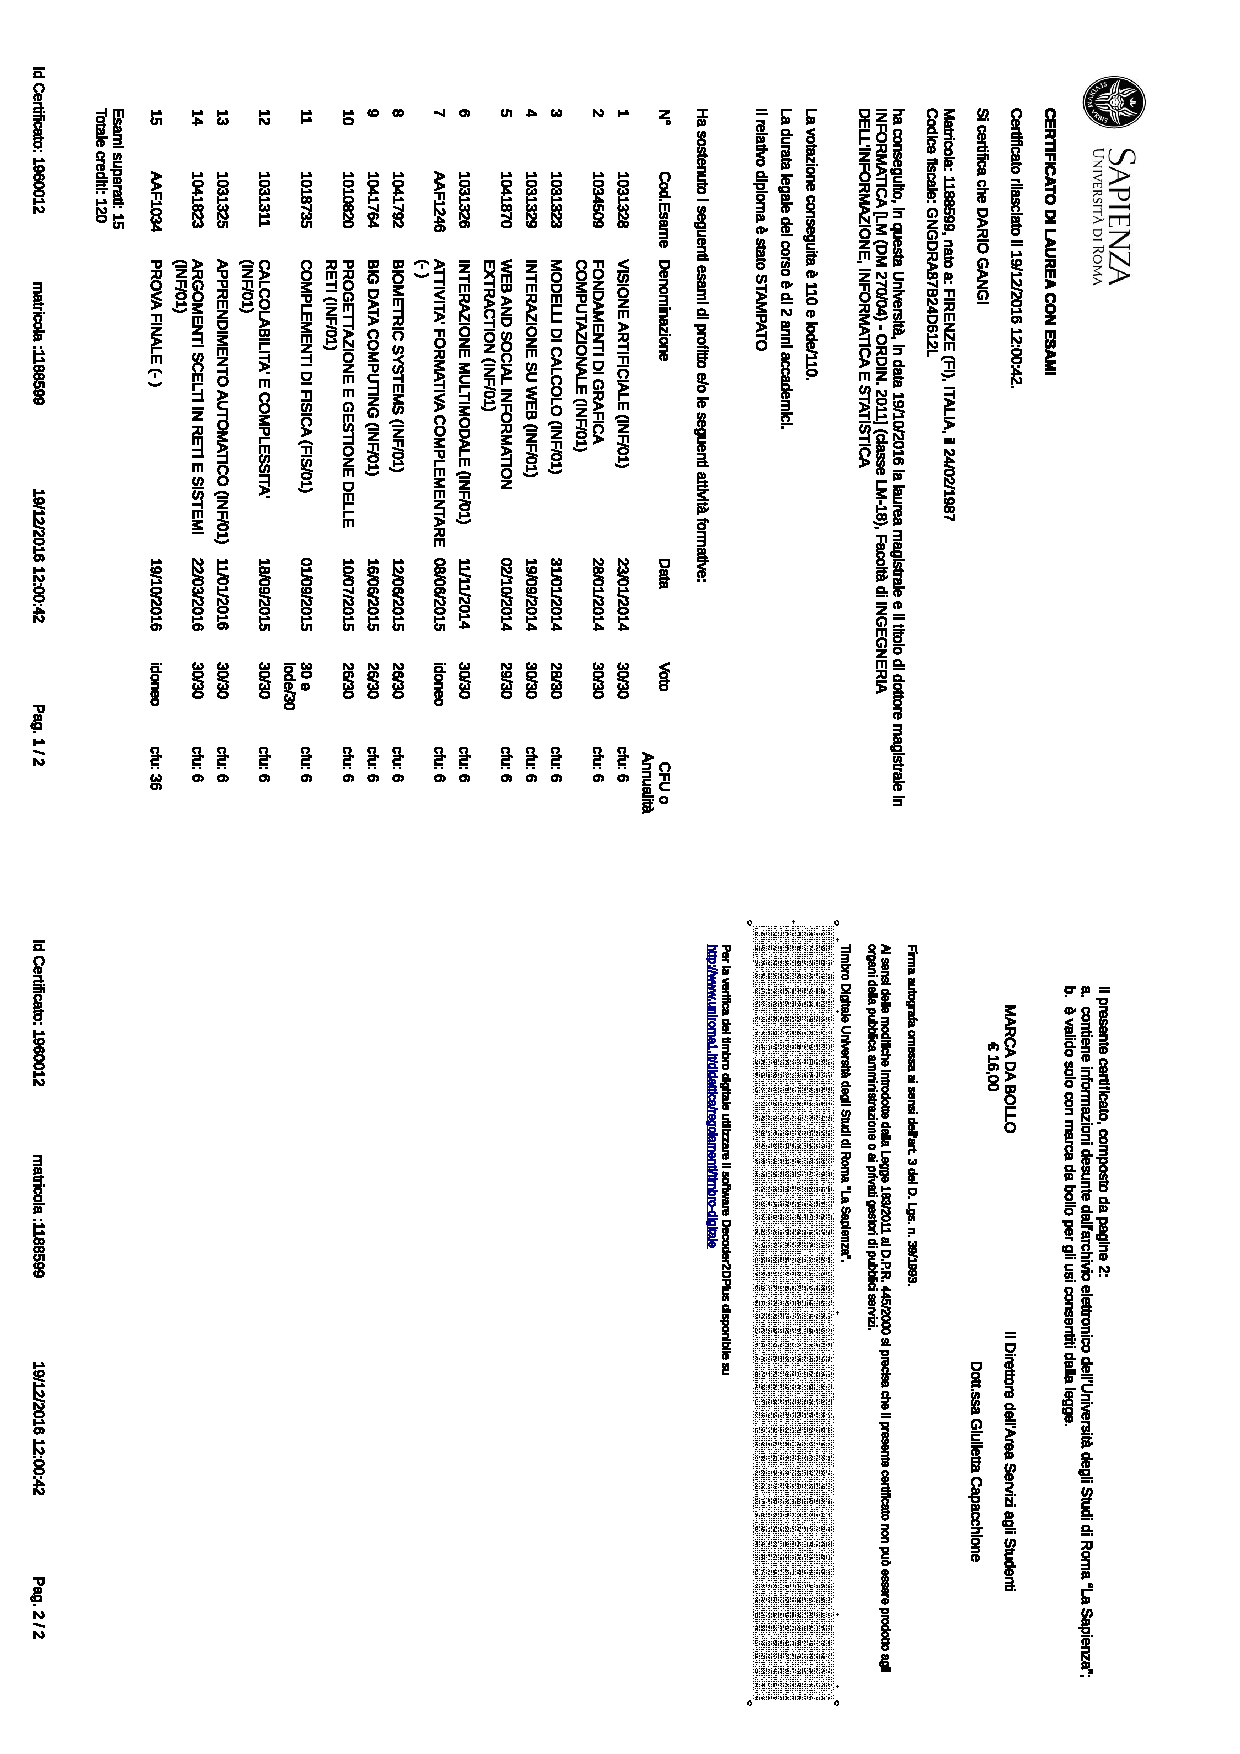
\includepdf[pages=-]{CertificatoLaureaMagistraleConEsami_multipagina.pdf}
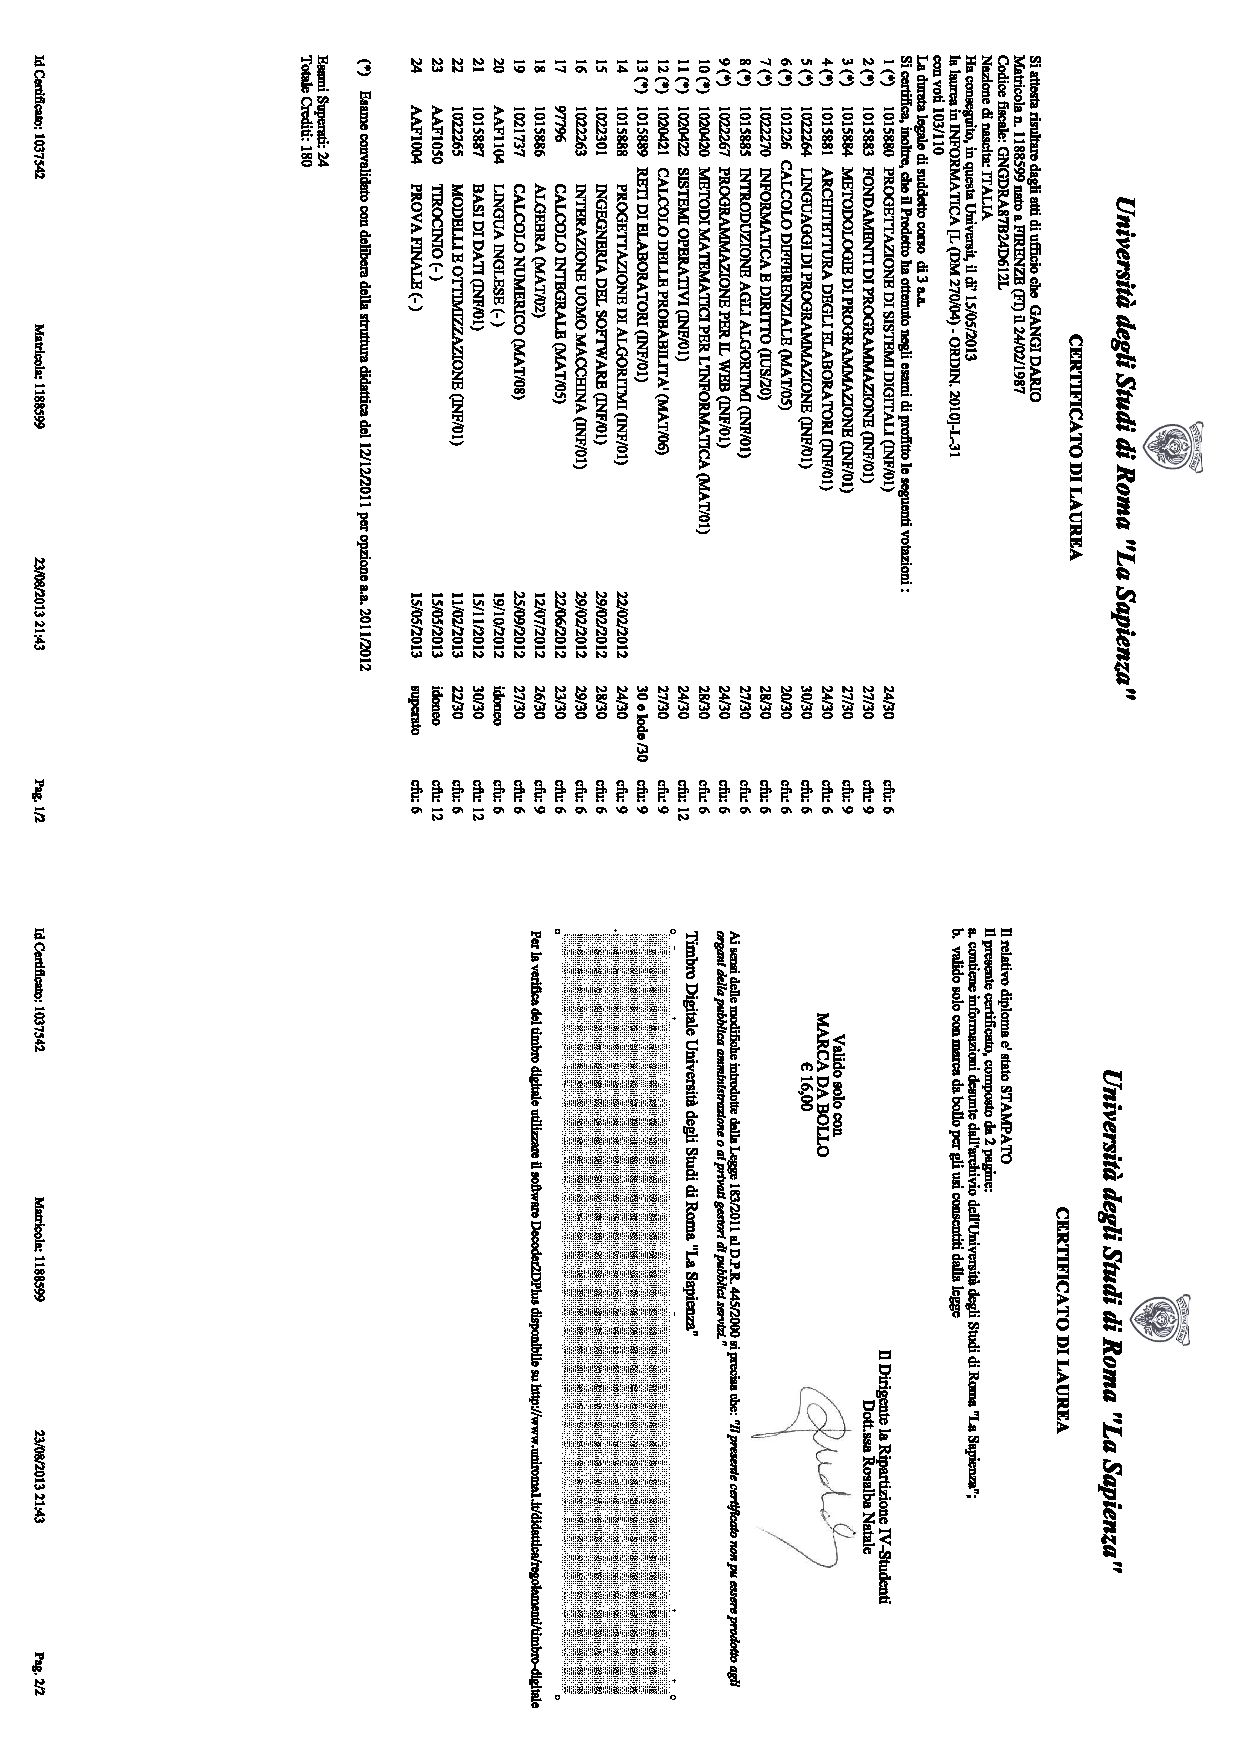
\includepdf[pages=-]{CertificatoLaureaConEsami_multipagina.pdf}
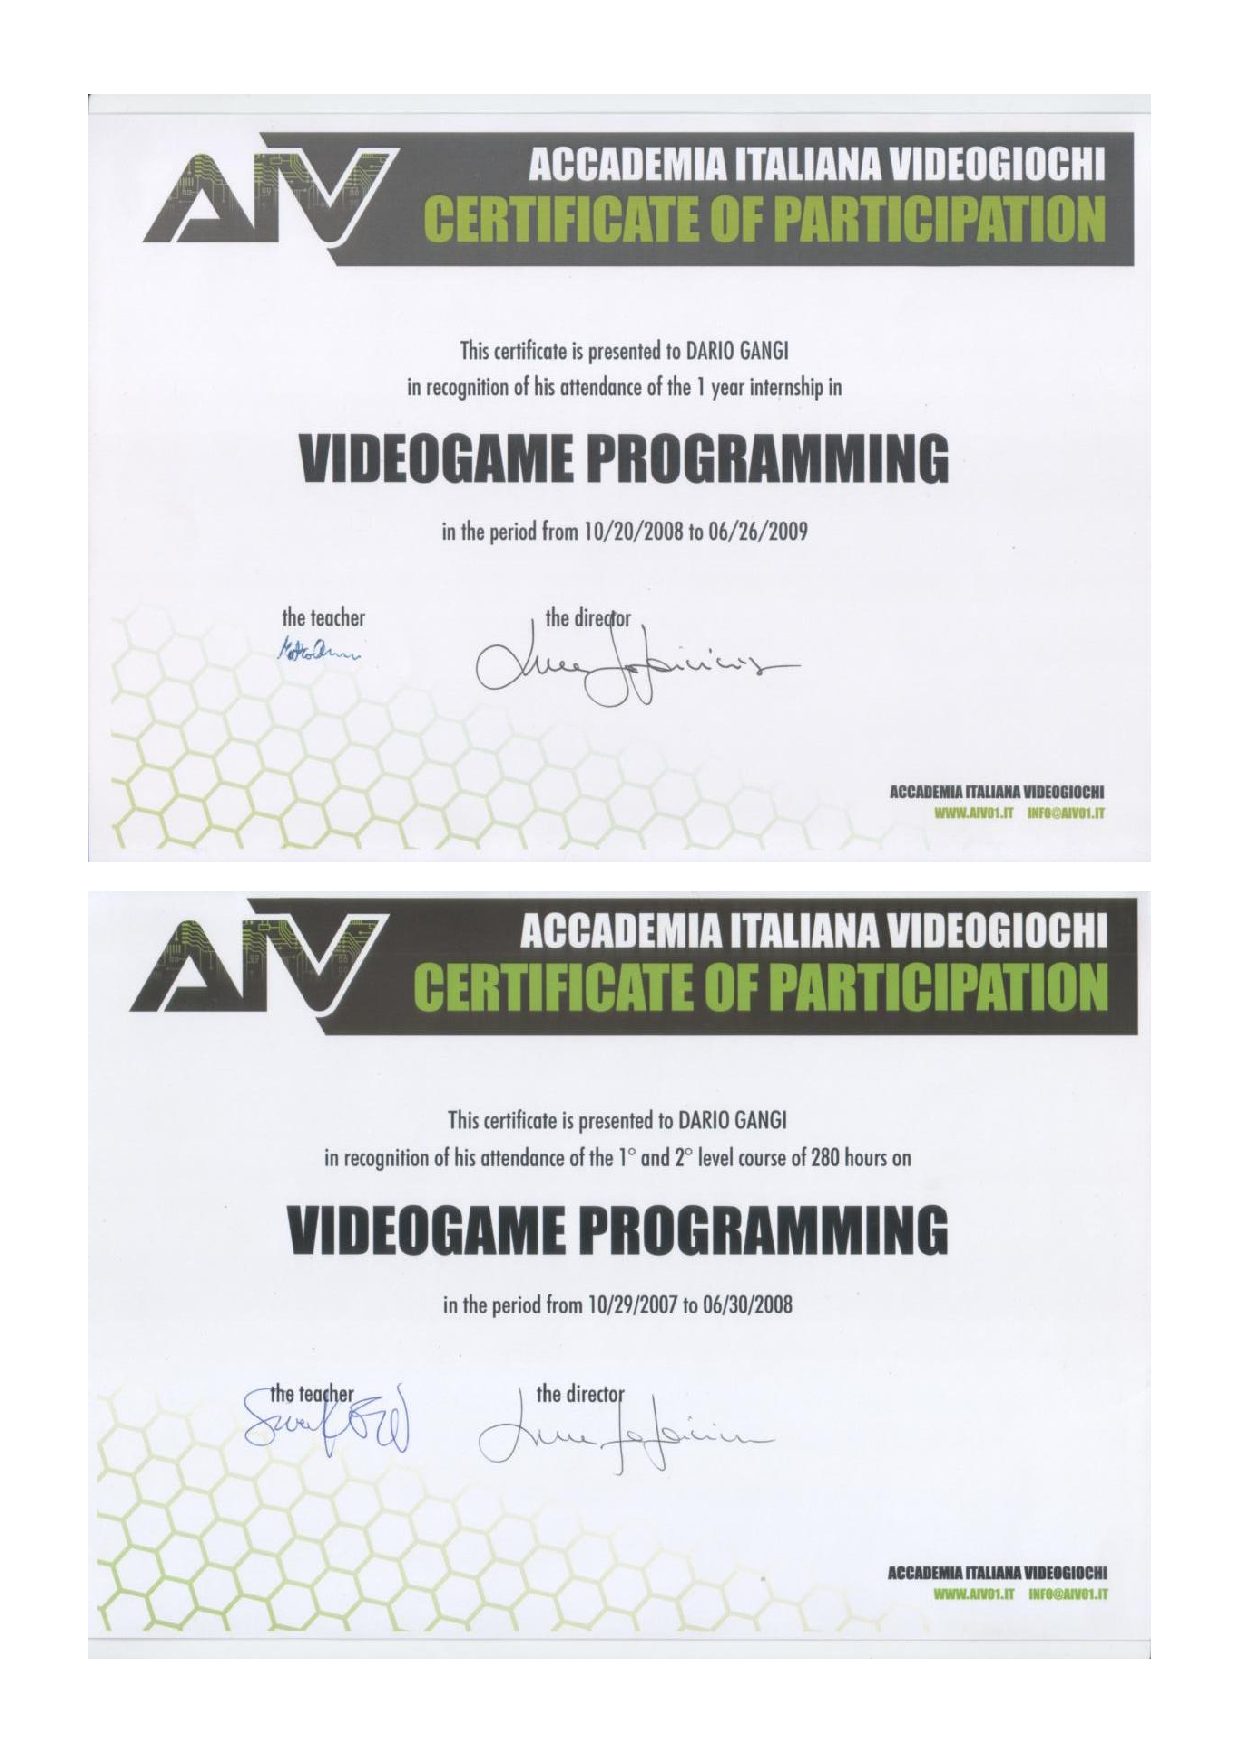
\includepdf[pages=-]{attestatoAIV.pdf}



\end{document}